\subsection{Context}
Drones, or UAVs, are not new technologies. UAVs are currently used extensively, for both offensive\cite{ref:offence} and defensive\cite{ref:defence} operations, by militaries across the globe. There is also a strong push for UAVs in commercial applications, such as package delivery\cite{ref:package} and agriculture\cite{ref:agriculture}, and an ever-growing population of hobbyists\cite{ref:hobby}, adventurers\cite{ref:adventure} and athletes\cite{ref:sport} using drone-mounted cameras to capture everything from weddings to skiing down mountains. However, there are several applications where current drone technology just can't compete.\\

\todo[inline]{Add more negatives/problems}
Rotor-based aircraft like the DJI Phantom (Figure \ref{fig:dji}) are highly maneuverable, easy to control, and can be launched from almost any location, but as a result of their large power demands have very limited range/endurance. This makes them difficult to use in applications requiring long distance travel, such as package delivery.

\begin{figure}[!h]
	\centering
	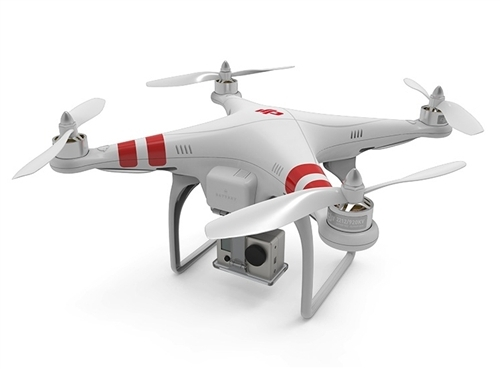
\includegraphics[width=150pt]{\IMAGEPATH /Aircraft/djiPhantom}
	\caption{DJI Phantom, a commercially available UAV}
	\label{fig:dji}
\end{figure}

\todo[inline]{Add more negatives/problems}
Wing-based aircraft such as those based on the Skywalker X8 frame (Figure \ref{fig:x8}) can achieve much greater travel distances as a result of higher efficiency flight. However, winged aircraft require open spaces to land safely, making them difficult to use in cramped or obstacle-rich applications such as low-altitude search near cities or forests.

\begin{figure}[!h]
	\centering
	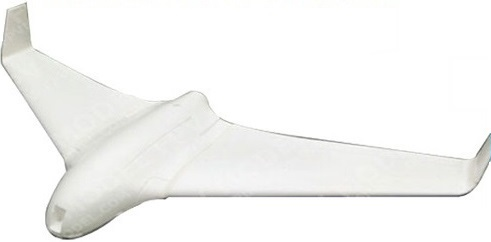
\includegraphics[width=160pt]{\IMAGEPATH /Aircraft/x8}
	\caption{Skywalker X8 airframe, a popular hobbyist choice}
	\label{fig:x8}
\end{figure}
 
The UAV Challenge\cite{ref:challenge} is a competition organised by the Queensland University of Technology and the CSIRO, held every 2 years to push the boundaries of current autonomous aircraft technology. The 2016 challenge is titled ``Medical Express'', and seeks to overcome some of the issues raised above. The objectives of the 2016 Challenge are to use unmanned aircraft to assist in a medical emergency.\\

Competitors must develop an aircraft than can fly to a known location (up to 30km) through specific transit corridors, search for and correctly identify ``Outback Joe'', land close to him to accept a pre-prepared blood sample, and then fly back to base. All of these actions must be completed within one hour, and must be autonomous; that is, after receiving the ``start'' signal the aircraft must have no human input.\\

The time period of the competition extends from registration (before 2nd September, 2015) to the final competition (week starting 19th of September, 2016), spanning over 1 year. Table \ref{tab:challenge} highlights the key dates and corresponding stages of the UAV Challenge.\\

\begin{table}[!ht]
	\caption{UAV Challenge Timeline}
	\label{tab:challenge}
	\centering
	\begin{tabular}{ | l | l | }
		\hline
		\textbf{Events} & \textbf{Date} \\ \hline \hline
		Registration and Deliverable 1: Short Technical Report & \textit{Completed} \\ \hline
		Deliverable 2: Technical Report and Video & 13th April 2016 \\ \hline
		Deliverable 3: Autonomous Flight Record & 3rd August 2016 \\ \hline
		Final ``Go/No-Go'' decision for teams & 10th August 2016 \\ \hline
		Medical Express Challenge & Week starting 19th September 2016 \\
		\hline
	\end{tabular}
\end{table}

\subsection{Project Outline}
This project involves the development of an autonomous Unmanned Aerial Vehicle (UAV) with the capabilities to compete in the 2016 UAV Challenge. From the task specified above, a number of design and performance requirements were identified for any aircraft to be successful in the Challenge:
\begin{enumerate}[label=\bfseries R\arabic*:] \itemsep-2pt
	\item Capacity to switch between automated and manual flight modes through user commands
	\item Ability to receive payload upon landing
	\item Take-off and landing in obstacle-rich environments (i.e. without runway)
	\item Total flight travel distance of at least 60km
	\item Total flight duration of at least 60 minutes
	\item Automated in-flight identification of a target
\end{enumerate}

\todo[inline]{Might remove some of these in final}
It is anticipated that there will be several Capstone student teams continuing development of the UAV in 2016. Given the requirements listed above, and the timeline of the Challenge, this project sought to develop a working prototype with which to achieve the basic functionality required to compete in the Challenge. As such, the following objectives were selected for the project:
\begin{enumerate}[label=\bfseries O\arabic*:] \itemsep-2pt
	\item Register for the 2016 UAV Challenge
	\item Provide a Bill of Materials for UAV development
	\item Development of a novel hybrid flight system, incorporating both Vertical Take-Off and Landing (VTOL) and Fixed-Wing flight modes, to achieve \textbf{R3}, \textbf{R4} and \textbf{R5}
	\item Development, documentation and implementation of autonomous flight controls
	\item Development of a low-cost, medium-range sensor system to enable object detection and path planning
	\item Development of in-flight search and obstacle avoidance mechanisms to achieve \textbf{R6}
	\item Establish a strong foundation for Capstone student teams to continue work in 2016
\end{enumerate}

The remaining sections of the report will discuss the work conducted by \ID in developing a working prototype for the UAV Challenge, beginning with formulating design requirements and constraints from the UAV Challenge specification. The following sections will discuss the various domains of the aircraft, including design, flight and planning systems, and sensing systems, with a particular focus on the novel transition system for hybrid flight. The report will end with conclusions and recommendations for future work.